%! Author = aaronspaulding
%! Date = 12/16/23


\subsection{An implementation of a Finite Difference Navier-Stokes solver to simulate the two-dimensional cylinder wake flow.}
I implemented a solver for the Navier-Stokes equations using a Finite Difference(FD) method.
This approach allows us to simulate fluid flows in two dimensions quickly and has been applied to many fluid related problems such as weather prediction, aerodynamics, and oceanography.
I implemented this solver in python using the NumPy library for efficient array computations.
The solver initializes the velocity and pressure fields and tracks changes and interactions between ``parcels'' of fluid interacting with each other.
Each parcel is stationary and has a velocity and pressure associated with it that is updated at each time step to track the flux into and out of the parcel.
This solver type enables efficient quick simulations at the cost of using fixed time steps and a fixed grid size.


\subsubsection{Environment Setup}
I designed the solver environment to be flexible and modular so users could easily define different size and resolution environments.
The environment has a customizable grid, with adjustable resolution, time step, and fluid properties.
This was implemented as a python ``Environment'' Class inside a module.
The ``Environment'' class also includes automatic plotting routines that enable quick visualization of the fluid flow.

\subsubsection{Boundary Conditions}
To extend this modularity I abstracted different types of boundary conditions common in fluid simulations.
I implemented four different boundary conditions for each edge of the environment.
Each of these boundary conditions is fully modular and can be mixed and matched for each simulation environment.

\begin{enumerate}
    \item \textbf{No-Slip Boundary Condition}: This boundary condition is used to simulate a solid boundary where fluid flows are zero in both the parallel and perpendicular directions to the boundary. This is seen on the inside of pipes, along buildings and objects, and against the ground.
    \item \textbf{Fixed Velocity Boundary Condition}: This boundary condition is used to simulate a boundary where fluid flows are fixed in the parallel direction to the boundary. This could be used to simulate a fan, an inlent valve, or the top of a boundary layer where the fluid is moving at a constant velocity.
    \item \textbf{Periodic Boundary Condition}: This boundary condition is used to simulate a boundary where fluid flows are periodic in the parallel direction to the boundary. This can be used to simulate repeating simulations such as a section of pipe where the input and output ends are similar.
    \item \textbf{Free Slip Boundary Condition}: This boundary condition is used to simulate a boundary where fluid flows are zero in the perpendicular direction to the boundary. This can be used to simulate a boundary where the fluid is free to move in the parallel direction but cannot move in the perpendicular direction.
\end{enumerate}


\subsubsection{Objects in the Environment}
Objects inside environments also interact with fluid flows and affect the velocity and pressure fields.
To enable modular simulations, I also implemented an ``Object'' Class that can be used to place arbitrary objects in the environment.
I implemented a ``Rectangle'' Class that inherits from the abstract ``Object'' Class that automatically manages boundary conditions of the added object and updates the velocity and pressure fields during simulation.
I also implemented a ``Cylinder'' Class that also inherits from the abstract ``Object'' Class.

These can be combined to make complex simulations with multiple objects interacting with each other and the fluid flow.

\subsubsection{Example Simulation Setup}
\begin{verbatim}
\inputminted{python}{examples/box_example.py}
\end{verbatim}

\begin{figure}[h]
    \centering
    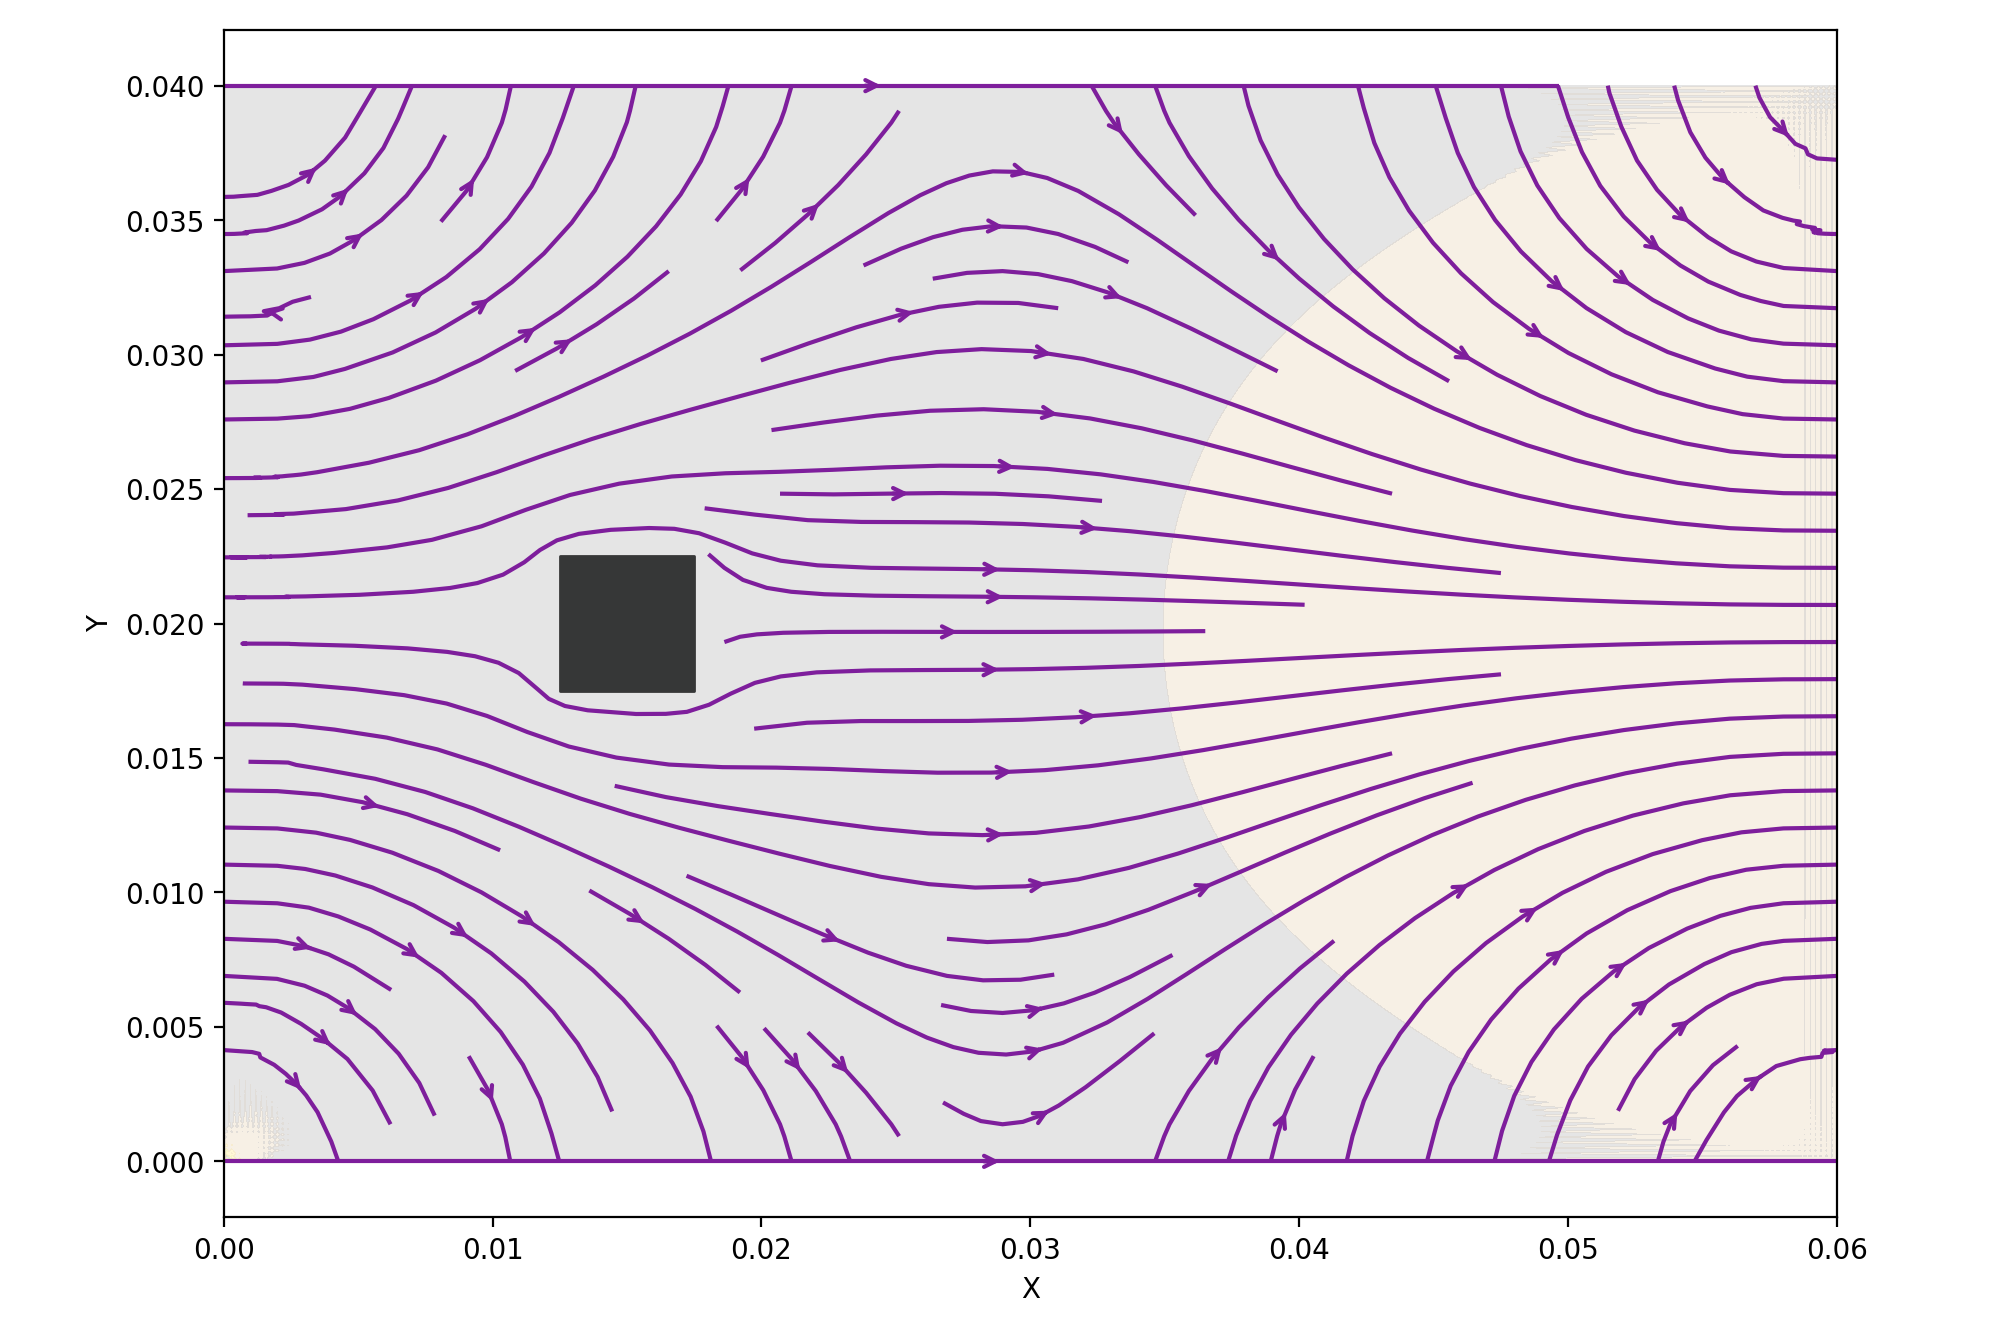
\includegraphics[width=0.5\linewidth]{Figures/box_example_streamline.png}
    \caption{Example streamline plot of a fluid flow around a box.}
    \label{fig:box_example_streamline}
\end{figure}


\subsection{Unit testing}
% TODO: Write this

\subsubsection{Automated Unit Testing with GitHub Actions}
% TODO: Write this

\section{Simulation of a fluid flow around a cylinder}